%\tiny
%\scriptsize
%\footnotesize
%\small

% 最後に句読点の変換を行うこと。全角ー>全角
%	。を.
%	、を,

%\documentclass[submit,techrep]{ipsj}
%\documentclass[submit,techrep,noauthor]{ipsj}
\documentclass[submit,techrep,noauthor]{ipsj}

%\usepackage[dvips]{graphicx}
\usepackage[dvipdfmx]{graphicx,hyperref}
\usepackage{latexsym}
\usepackage{color}
\definecolor{BLUE}{rgb}{0.00, 0.00, 1.00}
\usepackage{listings}
\lstset{
language={C},
%basicstyle={\ttfamily},
basicstyle={\footnotesize},
numbers=left,
stepnumber=1,
breaklines=true,
lineskip=-0.5mm,
%xleftmargin=2zw,
frame={tb}, 
showtabs=false,
%formfeed={\hfill},
}
\usepackage{cite}
%	\usepackage{comment}
%	\usepackage{caption}
\def\newblock{\hskip .11em plus .33em minus .07em}

\def\Underline{\setbox0\hbox\bgroup\let\\\endUnderline}
\def\endUnderline{\vphantom{y}\egroup\smash{\underline{\box0}}\\}
\def\|{\verb|}

\setcounter{巻数}{53}%vol53=2012
\setcounter{号数}{10}
\setcounter{page}{1}


\begin{document}


\title{PMlibを用いた計算性能測定と性能可視化手法}

\affiliate{AICS}{理化学研究所 計算科学研究機構}
\affiliate{Kyushu}{九州大学 情報基盤研究開発センター}

\author{三上 和徳}{Kazunori Mikami}{AICS}[kazunori.mikami@riken.jp]
\author{小野 謙二}{Kenji Ono}{Kyushu}

\begin{abstract}
オープンソースライブラリPMlib
を用いたアプリケーションの性能評価手法について報告する。
HPCシステムの仕様上の最大計算性能と
アプリケーション実行時に達成される実行性能との違いが頻繁に指摘される。
この違いを議論する場合には、演算器の並列性やメモリ階層における局所性確保などの
ハードウエアの動作特性を中心に評価する視点と、
アプリケーションがソースプログラムレベルで要求する数値計算上の計算量と
コンピュータシステムが実際に実行する命令に基づいた計算量との違いを
評価する視点の双方が必要である。

PMlibは数値計算上の計算量を明示的に測定する機能と、HWPCが記録する計算量を
測定する機能とを有し、両者の違いを定量的に評価することを可能とする。
またHWPC測定時には内部でPAPI低レベルAPIを利用し、
一般に選択と解釈が容易ではない各種ハードウエアイベント統計情報を
カテゴリ分けしてアプリ利用者が評価しやすい情報として選択出力する。

{ \color{BLUE}
出力情報としてはアプリ実行中に蓄積された統計情報を時間平均化した
標準レポートに加え、
経過時間軸に沿った動的な情報の出力も可能であり、
計算性能の時系列挙動を可視化するWebブラウザパッケージとの連携利用
が可能な構成となっている。(この報告は次回報告にまわすことにする)
}

これらの異なる基準での計算量・計算性能を評価することによって、
アプリケーションのHPCシステムにおける実行性能発現を理解する
一助とすることが可能である。

本報告ではPMlibを用いたアプリの性能評価手法を説明し、Intel Xeonサーバ
および富士通FX100上での評価事例を紹介する。
\end{abstract}

\maketitle

%1
\section{はじめに}
研究の目的

計算科学アプリケーションの開発および利用の各局面において、
利用するHPCシステム上で性能評価作業を実施することが頻繁に行われる。
これは主に、アプリケーションの性能特性を把握した後、ソフトウエア上の
最適化を実施して高速処理を実現するための可能性を探るために行われる。
このような性能評価作業が頻繁に実施される背景として、
HPCシステムの仕様上の最大性能とアプリケーションが実際に達成する実行性能との
差が、アプリの種類によっては非常に大きいことがある。

最大性能と実行性能との違いに関して
演算器の並列性やメモリおよびキャッシュ階層構成における局所性などの
ハードウエアの動作特性と関連づけられて
多くの研究が行われている。
一方、アプリケーションがソースプログラムレベルで要求する数値計算上の計算量と、
コンピュータシステムが実際に実行する命令を HWPC(ハードウエア性能カウンタ)
で測定した計算量との間でもしばしば大きな乖離がある。
この事は性能評価において重要な問題点として考慮されなければならない。

{ \color{BLUE}
例えば除算計算などはコンピュータシステムが実際に実行する命令ベースでの
(HWPCによる見かけ上の)実行性能が非常に高く表示されるが、
数値計算上(ソースプログラムで計上した)の計算量に基づく性能は一般に低い。
}

PMlibは数値計算上の計算量を明示的に測定する機能と、HWPCが記録する計算量を
測定する機能とを有し、両者の違いを定量的に評価することを可能とする。
HWPC測定には内部でPAPI低レベルAPIを利用し、
一般に選択と解釈が容易ではない各種ハードウエアイベント統計情報を
カテゴリ分けしてアプリ利用者が評価しやすい情報として選択出力する。
出力情報としてはアプリ実行中に蓄積された統計情報を時間平均化した
標準レポートに加え、
経過時間軸に沿った動的な情報の出力も可能であり、
計算性能の時系列挙動を可視化するWebブラウザパッケージとの連携利用
が可能な構成となっている。


\subsection {計算科学的観点での性能}
計算量という用語を用いる場合、計算科学アプリケーションの開発者は
Fortran言語やC++言語などで記述されたソースプログラム上で計上される
数値計算量をアプリケーションの計算量として認識することが多い。
計算科学的観点での計算性能とはこの計算量を計算経過時間で割った値として
定義される。

{ \color{BLUE}
以下式(単純結合式)は整理した後で書き直すこと。\\
%\begin{math} *** \end{math}
\begin{math}
Volume_{source} = \#add + \#mult + \#sub + \#div + \#sqrt + \#max + ...
\end{math}\\
\begin{math}
Perf_{source} = Volume_{source} \div Time
\end{math}\\
... みたいな?式が整理できた後で書き直す。\\
}

HPCアプリケーションにおいて
所与の計算を効果的に達成するために計算時間の短縮をめざす場合、
必要な計算量を削減するアルゴリズムを開発・採用するというアプローチ
が多いが、そのような場合の計算量とは主に上記が意図される。


\subsection {システム評価的観点での性能}

アプリケーションをHPCシステム上で実行する段階では、
ソースプログラムを言語コンパイラを通して生成した実行プログラムの
機械語命令列としてスケジューリング処理することになる。

ソースプログラムでは単純な計算式であっても、実際に実行されるのは
複数の命令列であり、計算量(例えば浮動小数点演算量)として
測定した場合、計算科学的観点での計算量と比較して多くなる。

HPCシステムが実際に処理するこの計算量を経過時間で割った値が
システム評価的観点での計算性能として定義される。

この計算量を測定するためには、HPCシステムに通常装備されている
HWPC(Hardware Performance Counter)に記録されるイベントカウント数
を利用することが可能である。
適切なAPIによってHWPCに記録された情報へアクセスし、
実行された命令数を測定して計算量を求める。

計算科学的観点で計算評価を行う場合、
ソースプログラムで記述される
平方根・三角関数といった数学関数ではそれぞれに計算の「重たさ」が異なる
ことは良く認識されているが、
四則演算や最小最大などの基本的な演算の「重たさ」も相当に異なることは
しばしば看過されがちである。


{ \color{BLUE}
線形結合式\\
\begin{math}
Volume_{system} = C_{1}\times \#add + C_{2}\times \#mult + C_{3}\times \#sub + C_{4}\times \#div + C_{5}\times \#sqrt + C_{6}\times \#max
\end{math}\\
... みたいな?式が整理できた後で書き直す。\\
}


(HWPCによる見かけ上の)実行性能が非常に高く表示されるが、
数値計算上(ソースプログラムで計上した)の計算量に基づく性能は一般に低い。

HWPCを基にした実行性能(FLOPS)、実効性能(%peak)
特定のシステム・アーキテクチャ・言語処理系SWでの性能に主眼がおかれる



\subsection {次行こう!}

性能情報の可視化 TRAiL

静的な統計情報の可視化
ジョブの経過時間で平均化された値

動的な性能挙動の可視化
ジョブの経過時刻に沿った過渡的な挙動
プロセス毎の過渡的な挙動
プロセス間の計算負荷バランスの挙動

本報告ではまず前段の、、、についていくつかの評価事例を通して
観点の違いによって評価量の測定値が大きく異なることを示したい。

性能測定値を時刻歴可視化することによって得られる、
性能挙動の理解に与える効果については、後続報告を行う計画である。

オープンソースライブラリPMlib \cite{PMlib1:webpage}。
オープンソースライブラリPMlib \cite{PMlib2:webpage}。

\begin{verbatim}
{
(1)PMlibとはどのようなツールか
・オープーンソース、C++クラスライブラリ、言語インタフェイス
・計算量の測定方法
・・ソースレベルでの明示的な指定、
・・・組み込み時の他ツールとの連絡(橋本ツール例)
・・HWPCによる採取
・・・HWPCのサポート状況
・測定した計算量の蓄積方法
・・逐次合算
・・時刻歴記録
・出力
・・テキストレポート
・・汎用トレースフォーマット(OTF)出力
}
\end{verbatim}

\section{PMlibの位置づけと関連研究}
性能評価に関するこれまでの研究とPMlibの位置づけ

\begin{verbatim}
{
アプリケーションの計算性能モニター用のライブラリ
オープンソース http://avr-aics-riken.github.io/PMlib
主な用途
タイマー、計算負荷の概要把握、HWPCへの簡易アクセスなど
利用方法
アプリのソース中に測定区間を指定。終了時に統計情報を出力
利用のモード
アプリに常時組み込み、プロダクション利用することを想定
性能測定・性能モデル化の支援にも期待
C++とFortranに対応するAPI 
特徴
インストールが簡単。講習会での実績平均10分
テキストレポートを基本とするコンパクトなツール
利用のための学習バリアが低い
}
\end{verbatim}

LinpackのFLOPSはソースで直接定義


rooflinemodel

OSやコンパイラなどの処理系に依存

オープンソース性能統計ツール類 {
Gprof: 簡易機能、コンパイラに制約
Scalasca: 高機能、Score-P共通インフラ
PAPI : HWPCへのアクセス
他 : 多数
}
ベンダーツール {
X86系
Intel
PGI
Sparc系
富士通
Oracle
Power系
}



測定可能な情報\\
{
既存ツールはほぼ全てが
サンプリングあるいはトレーシングによる測定で、性能の根拠は
HWPC情報を利用している
}

簡単さ\\
{
ベンダー製品の性能計測・統計ツール
○豊富な機能が統合化されたインタフェイス
○パッケージの完成度が高く、インストールが容易
○ 詳しいドキュメント、ベンダーによるサポート、安心感
△一般に高価格で相当の習熟期間が必要
△選択できるツールがシステム毎に制限される

オープンソースの性能計測・統計ツール
○各ツール毎に特徴・機能が明確
○様々なシステムへの移植可能
○価格の心配が不要
△ユーザーインタフェイスが個性的
△ものによりインストール・利用がそれなりに大変
}


\section{PMlibを用いた性能測定方法}


(2)PMlibでどのよう情報を得るか
・汎用タイマーとしての機能
・Fortran/C++で表記される数値計算上での演算量
・コンピュータが実行する命令ベースでのHW演算量

{ \color{BLUE}
発表スライドではCCA/EBT、OTF、HWPC(PAPI)を説明。そこに力点をおくとよい\\
}

(3)PMlibでどのような分析ができるか
・演算の種類毎に処理の「重たさ」を評価
・・浮動小数点四則演算、平方根や三角関数などの基本計算
・・・ー>コンピュータが見かけ上発揮する実行性能と、実際の数値計算性能との定量的な比較ができる
・・・ー>アプリのコーディングの指針に使える
・HWPCベースでのアーキテクチャの有効利用状況
・・使いやすい用にグループ化した統計出力
・・SSE/AVX系命令の実行比率
・・・ー>SIMD機構の有効利用の確認
・・キャッシュヒット率
・・・ー>コンパイラがどれだけ賢くコンピュータの能力を引き出しているか評価ができる
・・・ー>コンパイラオプションの選択、指示行の指定などで、どのような効果が現れるか


\section{PMlibを用いた性能測定と分析例}
・基本演算カーネル(+、*、*+、%、SQRTなど)
・ミニアプリ1例(NTChemかな)
・ピーク性能に対する実効性能比を裏付けてみる

{ \color{BLUE}
Skylakeの例で示すといい\\
ルーフラインモデルを示し、実測との比較を見るとよい\\
}

以下の\lstlistingname \ref{listing1}はPMlib APIを利用するFortranソースプログラムの例である。

%lstlistingのcaptionは思い通りについてくれないので手を抜いてみるw
%\begin{lstlisting}[caption={FortranプログラムへのPMlib組み込み例},label={listing1},captionpos=b]
%	\begin{lstlisting}[caption=strangeeffect,captionpos=t]
\begin{lstlisting}[caption={\hfill},label={listing1},captionpos=t]
program main
call f_pm_initialize (nWatch)
call f_pm_setproperties ("Koko!" icalc, iexcl)
call f_pm_start ("Koko!")
call mykernel (msize,n,a,b,c)
call f_pm_stop ("Koko!", fops, ncall)
call f_pm_print ("", isort)
call f_pm_printdetail ("", ilegend, isort)
end
\end{lstlisting}

\subsection{基本的な演算性能の評価}
\subsection{STREAM性能の評価}
STREAMベンチマーク\cite{stream:1995}
はコンピュータシステムのメモリバンド幅を測定するためのツールとして広く用いられている。
STREAMは変数配列の積和算(TRIAD)など、メモリread/write処理が主要な負荷となる
計算式の性能をアプリケーションプログラムレベルで測定出力する。
したがってその結果は「計算科学的観点」で評価された性能である。
このSTREAMプログラムを「システム評価的観点」で評価するとかなり様相が異なって来る。

まずSTREAMをSkylakeサーバ上で実行した場合の出力結果を示す。
Intelコンパイラのデフォルトオプションを用いている。
STREAM FortranプログラムOpenMPスレッド並列版を
1CPU上で8スレッド実行した場合、20スレッド実行した場合について示す。


Skylakeサーバ
されたHWPCベースでの
PMlibを用いて
メモリ階層での実測イベントベースによるデータ移動の状況を示す。
図


測定に用いたプラットフォーム
Intel Skylake CPU搭載サーバの構成と性能諸元表を以下に示す。\\
富士通prime HPC FX100構成と性能諸元表を以下に示す。\\
%\begin{figure}[tb]
%	\centering\includegraphics[width=0.45\textwidth]{figs/xeon-server-config.png}
%	\caption{figs/xeon-server-config.png}
%	\label{fig:stream-ivy-compact-1cpux8}
%\end{figure}



%\tiny
%\scriptsize
%\footnotesize
%\small
\begin{table}[tb]
\caption{サーバの構成(主にCPU部分)}
\label{tab:server-config}
\footnotesize
\begin{tabular}{l|c|c} \hline
system	&	FX100	&	Skylake	\\ \hline
CPU	&	SPARC64 VIIIifx	&	Gold 6148	\\ \hline
core GHz	&	1.975	&	2.4	\\ \hline
core peak Gflops	&	31.6	&	〜30	\\ \hline
L1\$	&	64KB/D+64KB/I	&	32KB/D+32KB/I	\\ \hline
L1D\$BW GB/s	&	140/R+70/W	&	154/R + 77/W	\\ \hline
\$ Linesize in Byte	&	256	&	64	\\ \hline
L2\$	&	-	&	1MB	\\ \hline
L2\$BW GB/s/core	&	-	&	154 ( ~70)	\\ \hline
LL\$ (size/cpu)	&	12MB	&	28MB(1.4MB/c)	\\ \hline
LL\$BW GB/s/core	&	70/R+35/W	&	77 ( ~43)	\\ \hline
Memory	&	HMC(8x16Ls)	&	DDR4-2666	\\ \hline
Mem GB/s/[CMGcpu]	&	120/R+120/W	&	128	\\ \hline
\#cores/[CMGcpu]	&	16	&	20	\\ \hline
\end{tabular}
\end{table}


Intelコンパイラにはオプションが多数あり、中でも特にメモリバンド幅に関係が深いと
思われる以下のオプションを組み合わせて比較した結果を
図\ref{fig:stream-ivy-compact-1cpux8} に示す。\\
{\color{BLUE}この図は仮置きでIvybridgeの結果。Skylakeの結果と差し替えること。}

\begin{figure}[tb]
\centering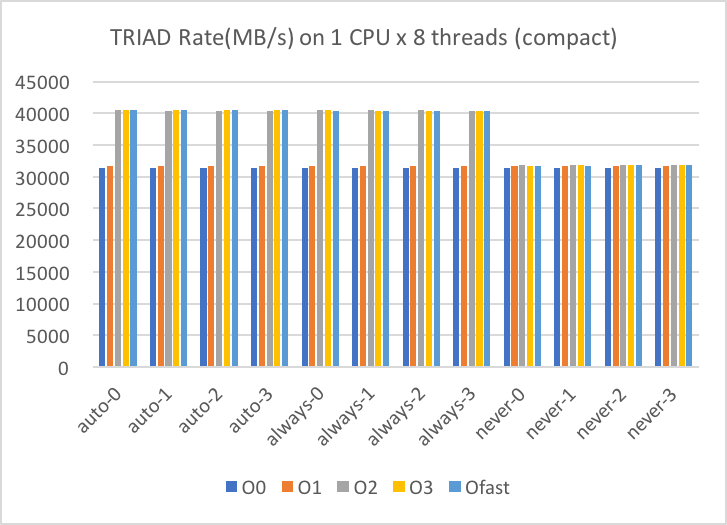
\includegraphics[width=0.45\textwidth]{figs/stream-ivy-compact-1cpux8.png}
\caption{stream-ivy-compact-1cpux8}
  \label{fig:stream-ivy-compact-1cpux8}
\end{figure}

{ \color{BLUE}
STREAM:Intel compilerでCache Eviction Levelオプションの指定効果はほとんど
なかった\\
}



\section{謝辞}

京補助金についての謝辞

\bibliographystyle{jplain}
\bibliography{main}

\end{document}
%%%%%%%%%%%%%%%%%%%%%%%%%%%%%%%%%%%%%%%%%%%%%%%%%%%%%%%%%%%%%%%%%%%%%%%%%%%%
%\begin{thebibliography}{10}
%
%\bibitem{PMlib1:webpage}
%PMlib公開Webページ,
%\urlj{https://github.com/avr-aics-riken/PMlib/}
%
%\bibitem{PMlib2:webpage}
%(こちらを示したほうが良いのか?)\\
%PMlib開発リポジトリ,
%\urlj{http://avr-aics-riken.github.io/PMlib/}
%
%\bibitem{Katouda:2016}
%M.Katouda, A.~Naruse, Y.~Hirano, and T.~Nakajima.:
%Massively parallel algorithm and implementation of ri-mp2 energy
%  calculation for peta-scale many-core supercomputers.
%{\em J. Comput. Chem.}, Vol.~37, No.~12, pp. 5373--5378, 2013.
%
%\bibitem{stream:1995}
%McCalpin, John D., 1995:
%Memory Bandwidth and Machine Balance in Current High Performance Computers
%{\em IEEE Computer Society Technical Committee on Computer Architecture (TCCA) Newsletter}, December 1995.
%
%\bibitem{stream:results}
%McCalpin, John D.:
%STREAM: Sustainable Memory Bandwidth in High Performance Computers,
%a continually updated technical report (1991-2007), available at:
%\urlj{http://www.cs.virginia.edu/stream/}
%
%\end{thebibliography}
%
%
